\chapter{针对条件扩散模型的高效图像修复算法}
\section{本章引言}
在\cite{Inverse}中,主要采用如下图像修复算法   

\section{算法设计}
\subsection{后验估计}
通常为了获得后验证估计$p(y\mid x_t)$,我们可以将该条件概率分布写为如下形式
\begin{equation}
    p(y\mid x_t) = \int_{\mathbb{R}^n} p(x_0\mid x_t) p(y\mid x_0,x_t) dx_0,
\end{equation}
我们如果从以下角度来思考本问题,即通过逆向随机微分方程(\ref{reverse SDE conditional})先从$x_t$可以得到$x_0$, 再通过前向加噪模型(\ref{Forward model})得到$y$。根据以上模型的Markov性质可以得到
\begin{equation}
     p(y\mid x_0,x_t) = p(y\mid x_0).
\end{equation}
因此我们可以得到
\begin{equation}
    p(y\mid x_t) = \int_{\mathbb{R}^n} p(x_0\mid x_t) p(y\mid x_0) dx_0=\mathbb{E}\left[p(y\mid x_0)\mid x_t\right],
    \label{conditional posterior formula}
\end{equation}
在\cite{Inverse}中直接采用将$\hat{x}_0=\mathbb{E}\left[x_0\mid x_t\right]$带入\ref{conditional posterior formula}用来逼近真实的后验概率分布,而此逼近方法取决于前向加噪算子$H(\cdot)$的光滑性,以及随着$x$的维数上升其逼近效果也在逐渐下降,因此本文中采用更加精确的后验估计方法进行图像还原。     


为了得到对后验概率分布$p(y\mid x_t)$的逼近,根据\cite{pseudoinverse,ddrm}中的结论,通常可以假设条件可以分布$p(x_0\mid x_t)$可以用$\mathcal{N}(\hat{x}_0(x_t);\gamma_t^2 I)$
来逼近,其中$\gamma_t^2 = \frac{\sigma_t^2}{1+\sigma_t^2}$。则我们可以重新用$x_t$来表示$x_0$。我们可以把$x_0$ 用$\hat{x}_0(x_t) + \gamma \epsilon$ 来逼近,其中我们有$\epsilon\sim \mathcal{N}(0,I)$为服从标准高斯分布的随机变量。 在只考虑$\mathcal{H}$为线性算子的情形下,我们将$y$表示为
\begin{equation}
    y=H(x_0)+n = H(\hat{x}_0+\gamma_t \epsilon)+n = H\hat{x}_0 + (H\epsilon+n).
\end{equation}
根据高斯分布随机变量的可叠加性,$(H\epsilon+n)$仍为高斯分布随机变量,其分布可以表示为$\mathcal{N}(0,\gamma_t^2 H^{\top}H + \sigma_y^2 I)$。因此我们最后可以将$\nabla_{x_t}\log(p(y\mid x_t))$写为
\begin{equation}
  -\frac{1}{2} \nabla_{x_t} \bigg((H\hat{x}_0-y)^{\top}\left(\gamma_t^2 H^{\top}H + \sigma_y^2 I\right)^{-1}(H\hat{x}_0-y)\bigg)
\end{equation}
利用链式法则和线性算子的性质,最后可以将$\nabla_{x_t}\log(p(y\mid x_t))$写为
\begin{equation}
    -\left(\gamma_t^2 H^{\top}H + \sigma_y^2 I\right)^{-1}(H\hat{x}_0-y)\frac{\partial \hat{x}_0(x_t)}{\partial x_t}
\end{equation}

\subsection{更新迭代过程}
在\cite{Inverse}中使用如下算法来进行更新迭代,最后得到$\hat{x}_0$作为对原始图像的逼近。在每一步更新迭代中,采用两步进行。第一步,先利用预训练集得到在原始无条件分布下的score function,从而得到在无条件生成通过DDPM采样更新得到的$x_{i-1}^{\prime}$以及得到$\hat{x}_0$。 第二步, 得到通过$\nabla_{x_i}\log(y\mid \hat{x}_0)$来更新$x_{i-1}^{\prime}$得到$x_{i-1}$。具体算法流程图如下算法\ref{DPS algorithm }可见
\begin{breakablealgorithm}
\caption{DPS Algorithm }
\label{DPS algorithm }
    \begin{algorithmic}[1]
   \REQUIRE Input $N$, $y$, $\{\zeta_i\}_{i=1}^{N}$, $\{\Tilde{\sigma}_i\}_{i=1}^{T}$
   \STATE $X_{T}\sim \mathcal{N}(0,\boldsymbol{I})$
   \FOR{$i$ = $N$ to 0}
   \STATE Set $\hat{s}\xleftarrow{} s_{\theta}(x_i,i)$
   \STATE Set $\hat{x_0} \xleftarrow{} \frac{1}{\sqrt{\Bar{\alpha}_i}}\left(x_i+(1-\Bar{\alpha}_i)\hat{s}\right)$
   \STATE Simulate $z\sim \mathcal{N}(0,\boldsymbol{I})$
   \STATE Set $x^{\prime}_{i-1}\xleftarrow{} \frac{\sqrt{\alpha_i}\left(1-\bar{\alpha}_{i-1}\right)}{1-\bar{\alpha}_i} \boldsymbol{x}_i+\frac{\sqrt{\bar{\alpha}_{i-1}} \beta_i}{1-\bar{\alpha}_i} \hat{\boldsymbol{x}}_0+\Tilde{\sigma}_i {z} $
   \STATE Update $x_{i-1}\xleftarrow{} {x}_{i-1}^{\prime}-\zeta_i \nabla_{{x}_t}\left\|{y}-\mathcal{A}\left(\hat{{x}}_0\right)\right\|_2^2 $
   \ENDFOR
   \RETURN $\hat{x}_0$ 
    \end{algorithmic}
\end{breakablealgorithm}      

两步迭代主要利用了在条件生成下的逆向随机微分方程的结构
\begin{equation}
    dx = \left(f(x,t) - g^2(t)(\nabla_{x_t}\log(p(x_t)))+ \nabla_{x_t}\log(y\mid x(t))\right)+g(t)d\Tilde{w}.
\end{equation}
第一步先更新除了带$\nabla_{x_t}\log(y\mid x(t))$的项,接下来再单独更新$\nabla_{x_t}\log(y\mid x(t))$的项。理论上$\nabla_{x_t}\log(y\mid x(t))$可以写为$-\frac{1}{\sigma_y^2}\nabla_{x_t}\|y-H(\hat{x}_0(x_t))\|_2^2$的形式,但是为了保证稳定性常常需要再前面乘以一个步长$\zeta_t$来保证收敛性,而在\cite{Inverse}中该步长为根据数据集本身形式人工选取,具有不稳定性和一定的随机性,不一定为最优的参数选取。如果$\sigma_y$过大则会导致每次更新步长多大如果$\sigma_y$过小则会导致每次更新步长不明显,最终生成的图片不一定能够对应损坏图片。因此在本文中采取如下方法,我们首先对应每次更新$\nabla_{x_t}\log(y\mid x(t))$项的时候的步长设置为$\eta_i$, 以及我们从$x_{i-1}^{\prime}$生成$x_{i-1}$的时候采用如下生成方式
\begin{equation}
    x_{i-1} \xleftarrow{} x_{i-1}^{\prime} - \eta_i \nabla_{x_i}\sqrt{((H\hat{x}_0-y)^{\top}\left(\gamma_i^2 H^{\top}H + \sigma_y^2 I\right)^{-1}(H\hat{x}_0-y)\bigg)}.
\end{equation}
该方法的优势在于不需要对步长刻意设置,我们在本模型中直接取$\eta_i=1$, $i=1,2,\cdots,T$, 也具有较好的稳定性。 如果直接取所有$\gamma_i=0$, $i=1,2,\cdots, T$, 则该更新方法可以写为
\begin{equation}
       x_{i-1} \xleftarrow{} x_{i-1}^{\prime} - \eta_i \nabla_{x_i}\|y-H(\hat{x}_0)\|_2,
\end{equation}
对右式继续进行化简可得
\begin{align}
    x_{i-1}^{\prime} - \eta_i \nabla_{x_i}\|y-H(\hat{x}_0)\|_2 &=  x_{i-1}^{\prime} - \frac{\eta_i}{\|y-H(\hat{x}_0)\|_2} H^{\top}(H\hat{x}_0-y)\frac{\partial \hat{x}_0}{\partial x_i}\\
    & = x_{i-1}^{\prime} - {\eta_i} H^{\top}\frac{(H\hat{x}_0-y)}{\|H\hat{x}_0-y\|_2}\frac{\partial \hat{x}_0}{\partial x_i},
\end{align}
中间的第二项里面的$\frac{(H\hat{x}_0-y)}{\|H\hat{x}_0-y\|_2}$已经被标注化,从而$\eta_i$可以控制每次更新的幅度,在原来的算法中如果仅仅对$\nabla_{x_i}\|H\hat{x}_0-y\|_2^2$进行步长选取,当$\|H\hat{x}_0-y\|$ 已经足够小的时候则不再更新,可能会陷入局部最优的解。(例如最后得到的还原图像确实经过加噪模型可以得到损坏图像,但是与原图像有较大的区别)经过实验该更新方法也确实有更好的鲁棒性。 

\subsection{算法流程}
基于DPS算法,我们现在提出我们采用更高效率基于DDIM模型的算法。在本文的改进算法中,可以采用DDPM模型进行采样,也可以对DDPM的模型中的总步长进行分割进行切片采样。进一步,还可以利用DDIM方法来进行采样,原先使用DDPM采样方法需要进行1000步,在DDIM方法下只需要100步就可以获得质量相似的图像。本文所提出的算法流程图如下所示

\begin{breakablealgorithm}
\caption{Image Restoration Algorithm }
\label{ours algorithm }
    \begin{algorithmic}[1]
   \REQUIRE Input $T$, $y$, $\{\eta_k\}_{k=1}^{T}$, $\{\sigma_k\}_{k=1}^{T}$
   \REQUIRE Choose $\{\tau_k\}_{k=1}^{m}$ according to the sampling scheme
   \STATE $X_{T}\sim \mathcal{N}(0,\boldsymbol{I})$
   \FOR{$t=m$, $m-1$, $\cdots$, $0$}
   \STATE Set $\hat{s}\xleftarrow{} s_{\theta}(\tau_t,x_{\tau_t})$
   \STATE Set $\hat{x_0} \xleftarrow{} \frac{1}{\sqrt{\Bar{\alpha}_{\tau_t}}}\left(x_{\tau_t}+\Bar{\beta}_{\tau_t}\hat{s}\right)$
   \STATE Simulate $z\sim \mathcal{N}(0,\boldsymbol{I})$
   \STATE Set $x^{\prime}_{\tau_{t-1}}\xleftarrow{} \frac{\sqrt{\alpha_{\tau_t}}\left(1-\bar{\alpha}_{\tau_{t-1}}\right)}{1-\bar{\alpha}_{\tau_t}} \boldsymbol{x}_{\tau_t}+\frac{\sqrt{\bar{\alpha}_{\tau_{t-1}}} \beta_{\tau_t}}{1-\bar{\alpha}_{\tau_t}} \hat{\boldsymbol{x}}_0+\sigma_{y} {z} $
   \STATE Update $x_{\tau_{t-1}}\xleftarrow{} {x}_{\tau_{t-1}}^{\prime}-\eta_t \nabla_{x_{\tau_t}}\sqrt{((H\hat{x}_0-y)^{\top}\left(\gamma_{\tau_t}^2 H^{\top}H + \sigma_y^2 I\right)^{-1}(H\hat{x}_0-y)\bigg)}. $
   \ENDFOR
   \RETURN $\hat{x}_0$ 
    \end{algorithmic}
\end{breakablealgorithm}


\section{参数选取与模型设计}
为了实现加噪过程以及去噪过程,需要以下结构: 
\begin{itemize}
    \item 加噪模型,其中包括前向算子$H$和对于噪声$n$的刻画,在该实验中,我们主要对低分辨算子,图像损坏算子来进行实验, 同时我们仅考虑$n$服从高斯分布的情形,即$n\sim \mathcal{N}(0,\sigma^2 I)$,其中我们取$\sigma=0.05$。 
    \item Diffusion model设置, 对于任意数据集,我们均选取 \href{https://github.com/openai/guided-diffusion}{https://github.com/openai/guided-diffusion} 中的各个数据集的标准预训练集来加载预训练集,对于具体的扩散模型使用说明可见附录 \ref{appendix}。 
    \item  后验估计,即在已知$z_t$, $y$ 的情形下,给出对于$\nabla_{z_t}\log\left(q(y\mid z_t)\right)$的估计。 在本文实验中利用算法\ref{ours algorithm }进行后验证估计。
    \item 条件采样过程,即在即在已知$z_t$, $y$ 的情形下,给出采样得到$z_{t-1}$的过程。 在算法\ref{ours algorithm }中,不失一般性,我们取$\eta_i=1.0$, 该参数不需要刻意微调,一般设置在0.5-1.0均可以实现较好的图像生成效果。 
    \item 下游任务设置,在本项目中主要选取图像损坏 
  (Image Inpainting)、 超分辨率 (Super Resolution) 、 图像线性去模糊化 (Motion Deblurring) 和 图像非线性去模糊化 (Nonlinear Deblurring) 下游任务进行实验。其中对于线性去模糊化和非线性去模糊化下游任务中本文利用了github仓库 \href{https://github.com/VinAIResearch/blur-kernel-space-exploring}{https://github.com/VinAIResearch/blur-kernel-space-exploring} 和 \href{https://github.com/LeviBorodenko/motionblur}{https://github.com/LeviBorodenko/motionblur} 的实现方法。 
\end{itemize}



\section{实验结果}
首先,本文对FFHQ数据集进行测试,我们以图像修复任务 (Image Inpainting)进行可视化展现实验结果。在实验中我们首先采用随机加噪方法进行前向加噪,对于每个像素有30\%的概率损坏变成白噪声,如下图\ref{noised image 1}即为加噪后的图像。 
\begin{figure}[H]
  \centering
  \begin{minipage}[b]{0.3\linewidth}

\includegraphics[width=\linewidth]{Picture/input/00000.png}
    \caption{加噪图像1}
    \label{noised image 1}
  \end{minipage}
  \hspace{0.1cm} % Space between images
   \begin{minipage}[b]{0.3\linewidth}
    
\includegraphics[width=\linewidth]{Picture/label/00000.png}
    \caption{原始图像1}
    \label{original image 1 }
  \end{minipage}
\hspace{0.1cm}
  \begin{minipage}[b]{0.3\linewidth}
    
\includegraphics[width=\linewidth]{Picture/recon/00000.png}
    \caption{还原图像1}
    \label{inpainted image 1}
  \end{minipage}
\end{figure}

\begin{figure}[H]
  \centering
  \begin{minipage}[b]{0.3\linewidth}

\includegraphics[width=\linewidth]{Picture/input/00001.png}
    \caption{加噪图像2}
    \label{noised image 2}
  \end{minipage}
  \hspace{0.1cm} % Space between images
   \begin{minipage}[b]{0.3\linewidth}
    
\includegraphics[width=\linewidth]{Picture/label/00001.png}
    \caption{原始图像2}
    \label{original image 2}
  \end{minipage}
\hspace{0.1cm}
  \begin{minipage}[b]{0.3\linewidth}
    
\includegraphics[width=\linewidth]{Picture/recon/00001.png}
    \caption{还原图像2}
    \label{inpainted image 2}
  \end{minipage}
\end{figure}


\begin{figure}[H]
  \centering
  \begin{minipage}[b]{0.3\linewidth}

\includegraphics[width=\linewidth]{Picture/input/00002.png}
    \caption{加噪图像3}
    \label{noised image 3}
  \end{minipage}
  \hspace{0.1cm} % Space between images
   \begin{minipage}[b]{0.3\linewidth}
    
\includegraphics[width=\linewidth]{Picture/label/00002.png}
    \caption{原始图像3}
    \label{original image 3}
  \end{minipage}
\hspace{0.1cm}
  \begin{minipage}[b]{0.3\linewidth}
    
\includegraphics[width=\linewidth]{Picture/recon/00002.png}
    \caption{还原图像3}
    \label{inpainted image 3}
  \end{minipage}
\end{figure}
以及如下图\ref{noised image 4}即为整块损坏图像,本文同时给出图像修复的还原过程切片。 更多实验结果可见附录\ref{appendix}。 



\begin{figure}[H]
  \centering
  \begin{minipage}[b]{0.3\linewidth}

\includegraphics[width=\linewidth]{Picture/input/input_box.png}
    \caption{加噪图像4}
    \label{noised image 4}
  \end{minipage}
  \hspace{0.1cm} % Space between images
   \begin{minipage}[b]{0.3\linewidth}
    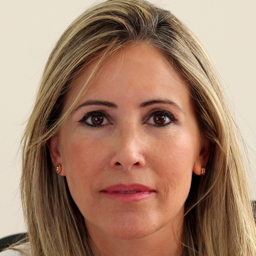
\includegraphics[width=\linewidth]{Picture/label/label_box.png}
    \caption{原始图像4}
    \label{original image 4}
  \end{minipage}
\hspace{0.1cm}
  \begin{minipage}[b]{0.3\linewidth}
    
\includegraphics[width=\linewidth]{Picture/recon/recon_box.png}
    \caption{还原图像4}
    \label{inpainted image 4}
  \end{minipage}
  \label{整块损坏图像}
\end{figure}


\begin{figure}[H]
  \centering
  \begin{minipage}[b]{0.3\linewidth}

\includegraphics[width=\linewidth]{Picture/progress/box/x_0500.png}
  \end{minipage}
  \hspace{0.1cm} % Space between images
   \begin{minipage}[b]{0.3\linewidth}
    
\includegraphics[width=\linewidth]{Picture/progress/box/x_0400.png}
  \end{minipage}
\hspace{0.1cm}
  \begin{minipage}[b]{0.3\linewidth}
    
\includegraphics[width=\linewidth]{Picture/progress/box/x_0200.png}
  \end{minipage}
\end{figure}

\begin{figure}[H]
  \centering
  \begin{minipage}[b]{0.3\linewidth}

\includegraphics[width=\linewidth]{Picture/progress/box/x_0500.png}
  \end{minipage}
  \hspace{0.1cm} % Space between images
   \begin{minipage}[b]{0.3\linewidth}
    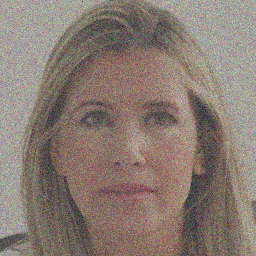
\includegraphics[width=\linewidth]{Picture/progress/box/x_0100.png}
  \end{minipage}
\hspace{0.1cm}
  \begin{minipage}[b]{0.3\linewidth}
    
\includegraphics[width=\linewidth]{Picture/progress/box/x_0000.png}
  \end{minipage}
\end{figure}




以下为在PSNR和SSIM两个度量下在不同图像修复算法下的表现,由此可以看到总体而言本文算法优于大部分图像修复算法,但是相比于在\cite{ddrm}中提出的DDRM算法仍然还有改善空间。 在图像修复任务(即Inpainting任务)中,本文所提出的算法相比于DPS算法有更好的表现,已经可以还原得到质量较高的图像。然而在整块损坏的图像修复任务中仍然不如DDRM\cite{ddrm}中所提出的算法,因为在整块挖去的情形下,对于后验分布估计相比于随机加噪的情形下无法利用损坏图像区域周围的像素点对图像进行充分还原。 
\begin{table}[H]
    \centering
    \begin{tabular}{|c|c|c|c|c|}
\hline \multirow[b]{2}{*}{ Method } & \multicolumn{2}{|c|}{ Inpaint (random)} & \multicolumn{2}{|c|}{ Inpaint (box) } \\
\hline & PSNR $\uparrow$ & $\operatorname{SSIM} \uparrow$ & PSNR $\uparrow$ & $\operatorname{SSIM} \uparrow$ \\
\hline \text{本文算法} & ${24.12}$ & $\underline{0.813}$ & \underline{18.95} & ${0.797}$ \\
\hline DPS\cite{Inverse}  & ${23.87}$ & ${0.781}$ & {18.90} & ${0.794}$ \\
\hline DDRM \cite{ddrm} & \underline{24.96} & 0.790 & ${18.66}$ & \underline{0.814} \\
\hline MCG\cite{MCG}  & 13.39 & 0.227 & 17.36 & 0.633 \\
\hline PnP-ADMM\cite{PnP}  & 23.75 & 0.761 & 12.70 & 0.657 \\
\hline \begin{tabular}{l} 
Score-SDE \cite{score_based_SDE} \\
\end{tabular} & 12.25 & 0.256 & 16.48 & 0.612 \\
\hline ADMM-TV & 22.17 & 0.679 & 17.96 & 0.785 \\
\hline
\end{tabular}
\caption{不同算法下的图像去噪结果}
\end{table}
以上为使用FFHQ数据集下进行图像修复的实验结果,总体而言在进行随机图像损坏任务中,在本文的算法改进下,在PSNR度量下优于DPS算法的图像修复结果,但是效果不如DDRM算法。但是考虑到DDRM算法在每一次反向迭代过程中需要每次对加噪算子$H$进行奇异值分解并且对图像逐元素进行更新, 因此在时间复杂度上不如本文提出的算法,以及在SSIM度量下本文的算法优于DDRM算法。 以及在对图像进行整块挖出的图像修复任务中,本文提出的算法在PSNR富相俩优于DPS算法,而在SSIM度量下仍然不如DDRM算法,这是由该任务的特性决定的。在对图像进行整块挖除的情形下,由于DDRM算法在对前向加噪算子进行起奇异值分解后,在逆向过程进行反向传播的过程中可以保留原图像的未损失图像的全部信息,对于整块挖除的损坏图像可以直接保留原始未损失图像。因此在DDRM算法下只需要对损坏区域单独进行修复即可,大大增加了图像修复的处理效率。 而在本文算法中,每一次迭代过程中将图像整体作为输入统一进行修复,而不对损坏区域进行特殊处理,因此相比而言在该任务下存在劣势。    


相比于在\cite{Inverse}中仅仅对FFHQ数据集进行测试,本文选择LSUN数据集中的Bedrooms卧室图像数据集进行测试,同样利用两种图像加噪方式 (随机加噪于整块挖除)进行实验,如下图为实验结果。此处我们选取了不同图像作为例子展现图像修复的还原过程。我们在图例中放了三张图像作为对比,最左边的是加噪后的图像,最中间的是原始图像作为ground truth和还原后的图像进行对比分析,最右边的图像为经过本文图像去噪算法后还原得到后的图像。 
\begin{figure}[H]
  \centering
  \begin{minipage}[b]{0.3\linewidth}
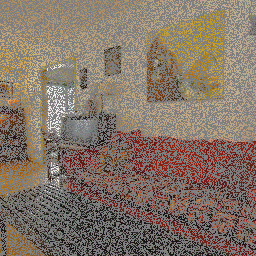
\includegraphics[width=\linewidth]{Picture/input/00007.png}
    \caption{加噪图像5}
    \label{noised image 5 }
  \end{minipage}
  \hspace{0.1cm} % Space between images
   \begin{minipage}[b]{0.3\linewidth}
    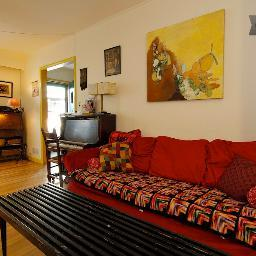
\includegraphics[width=\linewidth]{Picture/label/00007.png}
    \caption{原始图像5}
    \label{original image  5}
  \end{minipage}
\hspace{0.1cm}
  \begin{minipage}[b]{0.3\linewidth}
    
\includegraphics[width=\linewidth]{Picture/recon/00007.png}
    \caption{还原图像5}
    \label{inpainted image 5}
  \end{minipage}
  \label{整块损坏图像}
\end{figure}

\begin{figure}[H]
  \centering
  \begin{minipage}[b]{0.3\linewidth}

\includegraphics[width=\linewidth]{Picture/input/00008.png}
    \caption{加噪图像6}
    \label{noised image 6 }
  \end{minipage}
  \hspace{0.1cm} % Space between images
   \begin{minipage}[b]{0.3\linewidth}
    
\includegraphics[width=\linewidth]{Picture/label/00008.png}
    \caption{原始图像6}
    \label{original image 6}
  \end{minipage}
\hspace{0.1cm}
  \begin{minipage}[b]{0.3\linewidth}
    
\includegraphics[width=\linewidth]{Picture/recon/00008.png}
    \caption{还原图像6}
    \label{inpainted image 6}
  \end{minipage}
  \label{整块损坏图像}
\end{figure}


\begin{figure}[H]
  \centering
  \begin{minipage}[b]{0.3\linewidth}

\includegraphics[width=\linewidth]{Picture/input/00009.png}
    \caption{加噪图像7}
    \label{noised image 7 }
  \end{minipage}
  \hspace{0.1cm} % Space between images
   \begin{minipage}[b]{0.3\linewidth}
    
\includegraphics[width=\linewidth]{Picture/label/00009.png}
    \caption{原始图像7}
    \label{original image 7 }
  \end{minipage}
\hspace{0.1cm}
  \begin{minipage}[b]{0.3\linewidth}
    
\includegraphics[width=\linewidth]{Picture/recon/00009.png}
    \caption{还原图像7}
    \label{inpainted image 7}
  \end{minipage}
  \label{整块损坏图像}
\end{figure}



\begin{figure}[H]
  \centering
  \begin{minipage}[b]{0.3\linewidth}

\includegraphics[width=\linewidth]{Picture/input/00010.png}
    \caption{加噪图像8}
    \label{noised image  8}
  \end{minipage}
  \hspace{0.1cm} % Space between images
   \begin{minipage}[b]{0.3\linewidth}
    
\includegraphics[width=\linewidth]{Picture/label/00010.png}
    \caption{原始图像8}
    \label{original image 8 }
  \end{minipage}
\hspace{0.1cm}
  \begin{minipage}[b]{0.3\linewidth}
    
\includegraphics[width=\linewidth]{Picture/recon/00010.png}
    \caption{还原图像8}
    \label{inpainted image 8}
  \end{minipage}
  \label{整块损坏图像}
\end{figure}

\begin{figure}[H]
  \centering
  \begin{minipage}[b]{0.3\linewidth}

\includegraphics[width=\linewidth]{Picture/progress/random/x_0500.png}
  \end{minipage}
  \hspace{0.1cm} % Space between images
   \begin{minipage}[b]{0.3\linewidth}
    
\includegraphics[width=\linewidth]{Picture/progress/random/x_0400.png}
  \end{minipage}
\hspace{0.1cm}
  \begin{minipage}[b]{0.3\linewidth}
    
\includegraphics[width=\linewidth]{Picture/progress/random/x_0200.png}
  \end{minipage}
\end{figure}

\begin{figure}[H]
  \centering
  \begin{minipage}[b]{0.3\linewidth}

\includegraphics[width=\linewidth]{Picture/progress/random/x_0500.png}
  \end{minipage}
  \hspace{0.1cm} % Space between images
   \begin{minipage}[b]{0.3\linewidth}
    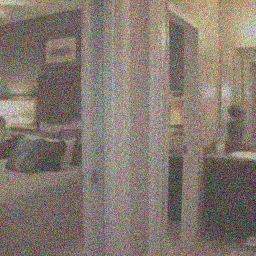
\includegraphics[width=\linewidth]{Picture/progress/random/x_0100.png}
  \end{minipage}
\hspace{0.1cm}
  \begin{minipage}[b]{0.3\linewidth}
    
\includegraphics[width=\linewidth]{Picture/progress/random/x_0000.png}
  \end{minipage}
\end{figure}

我们在FFHQ数据集上同时进行了更加丰富的实验,我们对不同图像均进行了图像修复操作,结果展示如下。 以下为在FFHQ数据集上测试的结果展示
\begin{figure}[H]
  \centering
  \begin{minipage}[b]{0.3\linewidth}
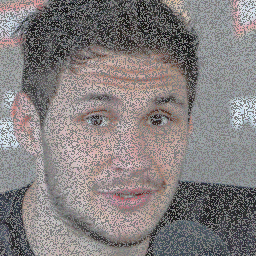
\includegraphics[width=\linewidth]{Picture/input/00004.png}
    \caption{加噪图像9}
    \label{noised image }
  \end{minipage}
  \hspace{0.1cm} % Space between images
   \begin{minipage}[b]{0.3\linewidth}
    
\includegraphics[width=\linewidth]{Picture/label/00004.png}
    \caption{原始图像9}
    \label{original image }
  \end{minipage}
\hspace{0.1cm}
  \begin{minipage}[b]{0.3\linewidth}
    
\includegraphics[width=\linewidth]{Picture/recon/00004.png}
    \caption{还原图像9}
    \label{inpainted image}
  \end{minipage}
\end{figure}



\begin{figure}[H]
  \centering
  \begin{minipage}[b]{0.3\linewidth}

\includegraphics[width=\linewidth]{Picture/input/00005.png}
    \caption{加噪图像10}
    \label{noised image }
  \end{minipage}
  \hspace{0.1cm} % Space between images
   \begin{minipage}[b]{0.3\linewidth}
    
\includegraphics[width=\linewidth]{Picture/label/00005.png}
    \caption{原始图像10}
    \label{original image }
  \end{minipage}
\hspace{0.1cm}
  \begin{minipage}[b]{0.3\linewidth}
    
\includegraphics[width=\linewidth]{Picture/recon/00005.png}
    \caption{还原图像10}
    \label{inpainted image}
  \end{minipage}
\end{figure}

\begin{figure}[H]
  \centering
  \begin{minipage}[b]{0.3\linewidth}
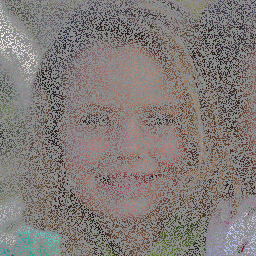
\includegraphics[width=\linewidth]{Picture/input/00006.png}
    \caption{加噪图像11}
    \label{noised image }
  \end{minipage}
  \hspace{0.1cm} % Space between images
   \begin{minipage}[b]{0.3\linewidth}
    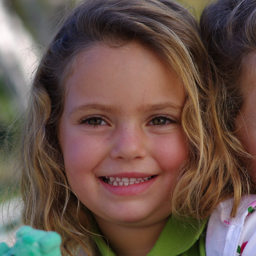
\includegraphics[width=\linewidth]{Picture/label/00006.png}
    \caption{原始图像11}
    \label{original image }
  \end{minipage}
\hspace{0.1cm}
  \begin{minipage}[b]{0.3\linewidth}
    
\includegraphics[width=\linewidth]{Picture/recon/00006.png}
    \caption{还原图像11}
    \label{inpainted image}
  \end{minipage}
\end{figure}


\section{更多结果}
本文所精心设计的图像还原算法展现出了卓越的泛化能力,这一能力使其能够轻松应对不同数据集下的图像还原任务。不论面对的是何种类型的图像数据,该算法都能够凭借其高效的运算机制,实现精准的图像还原效果。值得一提的是,这种算法的独特之处在于其对超参数的宽容性。在实际应用中,我们无需对超参数进行繁琐且精细的调整,算法便能够自动适应不同的图像特性,从而确保还原效果的稳定性和可靠性。    


为了进一步验证这一算法的实际效果,我们特别选取了两位国际一线篮球巨星的图像进行实验。这两位篮球巨星不仅在全球范围内拥有极高的知名度和影响力,他们的形象也因其独特的个人风格和比赛风采而深入人心。通过将这些篮球巨星的图像作为实验样本,我们能够更加直观地感受到该算法在图像还原方面的卓越性能。实验结果表明,无论是对于清晰度、色彩还原度还是细节表现,该算法都展现出了令人满意的效果,充分证明了其在实际应用中的价值和潜力。
\begin{figure}[H]
  \centering
  \begin{minipage}[b]{0.3\linewidth}

\includegraphics[width=\linewidth]{Picture/input/kun1_input.png}
  \end{minipage}
  \hspace{0.1cm} % Space between images
   \begin{minipage}[b]{0.3\linewidth}
    
\includegraphics[width=\linewidth]{Picture/label/kun1_label.png}
  \end{minipage}
\hspace{0.1cm}
  \begin{minipage}[b]{0.3\linewidth}
    
\includegraphics[width=\linewidth]{Picture/recon/kun1_recon.png}
  \end{minipage}
  \caption{球星图像修复1}
\end{figure}



\begin{figure}[H]
  \centering
  \begin{minipage}[b]{0.3\linewidth}

\includegraphics[width=\linewidth]{Picture/input/kun2_input.png}
  \end{minipage}
  \hspace{0.1cm} % Space between images
   \begin{minipage}[b]{0.3\linewidth}
    
\includegraphics[width=\linewidth]{Picture/label/kun2_label.png}
  \end{minipage}
\hspace{0.1cm}
  \begin{minipage}[b]{0.3\linewidth}
    \includegraphics[width=\linewidth]{Picture/recon/kun2_recon.png}
  \end{minipage}
  \caption{球星图像修复2}
\end{figure}


\begin{figure}[H]
  \centering
  \begin{minipage}[b]{0.3\linewidth}
\includegraphics[width=\linewidth]{Picture/input/mamba_input.png}
  \end{minipage}
  \hspace{0.1cm} % Space between images
   \begin{minipage}[b]{0.3\linewidth}
    \includegraphics[width=\linewidth]{Picture/label/mamba_label.png}
  \end{minipage}
\hspace{0.1cm}
  \begin{minipage}[b]{0.3\linewidth}
    \includegraphics[width=\linewidth]{Picture/recon/mamba_recon.png}
  \end{minipage}
  \caption{球星图像修复3}
\end{figure}




\section{本章小结}
